% Figure 3: mean kleos_policy score on the 349-item benchmark, base + orchestration (arm1)
% vs fine-tuned (arm2), with the recorded example-level 95% bootstrap intervals.
% source: pilot, docs/experiments.md H1 corrected scores (EXP:167): 0.4744 / 0.8015; no corrected
%   interval is recorded for the baseline, so neither pilot bar carries one.
% source: Hermes report (HER:259-262): arm1 0.4755 [0.4532-0.4978], arm2 0.8051 [0.7813-0.8288].
% source: Logos v0.0.1 report (L1:291-294): arm1 0.4469 [0.4219-0.4720], arm2 0.7896 [0.7644-0.8147].
% source: Logos v0.0.2, docs/experiments.md H9 result (EXP:790-791): arm2 0.8596, descriptive, no arm1.
% The error-bar lengths are the distances from each mean to its recorded interval endpoints.
\begin{figure}[t]
\centering
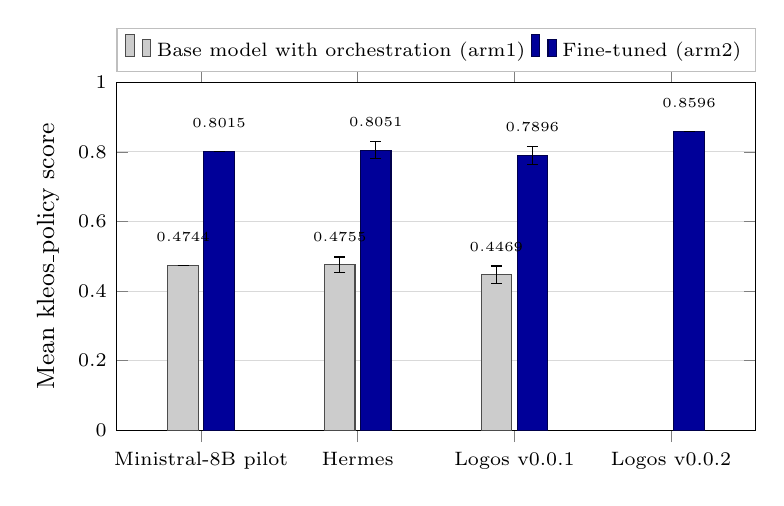
\begin{tikzpicture}
\begin{axis}[
  ybar, bar width=11pt,
  width=0.8\linewidth, height=6cm,
  ylabel={Mean \code{kleos\_policy} score}, ymin=0, ymax=1.0,
  symbolic x coords={Ministral-8B pilot, Hermes, Logos v0.0.1, Logos v0.0.2},
  xtick={Ministral-8B pilot, Hermes, Logos v0.0.1, Logos v0.0.2}, enlarge x limits=0.18,
  ytick={0,0.2,0.4,0.6,0.8,1.0},
  ymajorgrids, grid style={gray!30},
  legend style={at={(0.5,1.03)}, anchor=south, legend columns=2, font=\scriptsize, draw=gray!50}, legend cell align=left,
  tick label style={font=\scriptsize}, label style={font=\small},
  nodes near coords, nodes near coords style={font=\tiny, yshift=5pt, /pgf/number format/.cd, fixed, precision=4},
  error bars/y dir=both, error bars/y explicit,
  error bars/error bar style={black, thin},
]
\addplot[fill=gray!40, draw=gray!60!black] plot[error bars/.cd, y dir=both, y explicit] table[x=model, y=score, y error plus=ep, y error minus=em] {
model score ep em
{Ministral-8B pilot} 0.4744 0 0
{Hermes} 0.4755 0.0223 0.0223
{Logos v0.0.1} 0.4469 0.0251 0.0250
};
\addlegendentry{Base model with orchestration (arm1)}
\addplot[fill=blue!60!black, draw=blue!30!black] plot[error bars/.cd, y dir=both, y explicit] table[x=model, y=score, y error plus=ep, y error minus=em] {
model score ep em
{Ministral-8B pilot} 0.8015 0 0
{Hermes} 0.8051 0.0237 0.0238
{Logos v0.0.1} 0.7896 0.0251 0.0252
{Logos v0.0.2} 0.8596 0 0
};
\addlegendentry{Fine-tuned (arm2)}
\end{axis}
\end{tikzpicture}
\caption{Mean \code{kleos\_policy} score on the 349-item benchmark. Error bars are the recorded item-level 95\% bootstrap intervals (Hermes and Logos v0.0.1 only; the pilot baseline was re-graded after its interval was recorded, and the Logos v0.0.2 overall mean is descriptive). Logos v0.0.2 has no base arm. Item-level intervals treat the 349 items as independent and are narrower than the cluster intervals used from H8 on (Section~\ref{sec:protocol}).}
\label{fig:main}
\end{figure}
